\documentclass{beamer}

\usepackage{multicol}
\usepackage{float}

\usetheme[progressbar=frametitle]{metropolis}
\setbeamertemplate{frame numbering}[fraction]
\useinnertheme{metropolis}
\useoutertheme{metropolis}
\usefonttheme{metropolis}
\usecolortheme{spruce}
\setbeamercolor{background canvas}{bg=white}
%different themes are available
\definecolor{babyblueeyes}{rgb}{0.63, 0.79, 0.95}
%define custom theme using rgb, check latexcolor.com for information
\usecolortheme[named=babyblueeyes]{structure}


\title[Interacting Manifolds]{Magnetic Mirror Effect in Magnetron Plasma:}
\subtitle{Modeling of Plasma Parameters}


%may use macros to set new frame defaults

\setbeamercovered{transparent=25}
%hide onslide part by making it more transparent
%cant do this with only, but with onslide


\newcommand\myfigure[1]{%
	\medskip\noindent\begin{minipage}{\columnwidth}
		\centering%
		#1%
		%figure,caption, and label go here
	\end{minipage}\medskip}
\newcommand{\comment}[1]{}

\begin{document}
	\metroset{block=fill}
	%shades the background of a block
	
	%In beamer we create frames 1 frame= 1 page to hold our information
	\begin{frame}
		\titlepage	
	\end{frame}	
	
	\begin{frame}[t]{1.1 Density Function }
			$ f(x, y, z, v_{x}, v_{y}, v_{z}, t) :$ \\ number of particles at position $ (x, y, z) $ at time $ t $ with velocities between $ v_{x} $ and $ v_{x} + dv_{x} $, $ v_{y} $ and $ v_{y} + dv_{y} $, $ v_{z} $ and $ v_{z} + dv_{z} $ \\
			Notation: \\
			$ f(\textbf{r}, \textbf{v}, t) := f(x, y, z, v_{x}, v_{y}, v_{z}, t)$
			$$\displaystyle f(\textbf{r},t) = \int_{all \hspace{0.2cm} v_{x}^{}} dv_{x} \int_{all \hspace{0.2cm} v_{y}^{}} dv_{y} \int_{all \hspace{0.2cm} v_{z}^{}} dv_{z} f(\textbf{r}, \textbf{v}, t) $$
			Also written as
			$$\displaystyle \int_{all \hspace{0.2cm} \textbf{v}^{}} d^{3}v f(\textbf{r}, \textbf{v}, t) \hspace{0.5cm}\textrm{or} \hspace{0.5cm}\int_{all \hspace{0.2cm} \textbf{v}^{}} d\textbf{v} f(\textbf{r}, \textbf{v}, t)$$
			\end{frame}
		
	\begin{frame}[t]{Density function}
		Normalized density function denoted $ \hat{f}(\textbf{r}, \textbf{v}, t) $
		$$\displaystyle \int_{all \hspace{0.2cm} \textbf{v}^{}} d\textbf{v} f(\textbf{r}, \textbf{v}, t) = 1$$
		Average velocity
		$$\displaystyle \bar{v} = \int_{all \hspace{0.2cm} \textbf{v}^{}} d\textbf{v} \hspace{0.2cm} v \hspace{0.2cm} f(\textbf{r}, \textbf{v}, t)$$
		Other parameters \\
		Root Mean Square velocity $v_{rms}$ \\
		average absolute velocity $|\bar{v}|$ \\
		average velocity in $z$ direction $\bar{v_{z}}$
	\end{frame}
	
	\begin{frame}[t]{1.2 Maxwell Boltzmann Distribution} \vspace{10pt}
		Density Function
		\begin{equation}
			\label{eqn:maxwellian}
			\widehat{f_{M}}(\textbf{r}, \textbf{v}, t) = \left(\frac{m}{2\pi KT}\right)^{\frac{3}{2}} exp \left(-\frac{v^{2}}{v_{th}^{2}}\right)
		\end{equation}\\
	$$v_{th}^{2} = \frac{2 K T}{m}$$\\
	\vspace{30pt}
	Features of the Maxwell Boltzmann Distribution (Maxwellian)
	$$ v_{rms} = \sqrt{\frac{3 K T}{m}} \mathrm{,} |\bar{v}| = 2\sqrt{\frac{2 K T}{\pi m}} \mathrm{,} |\bar{v_{z}}| = \sqrt{\frac{2 K T}{\pi m}} \mathrm{,} \bar{v_{z}} = 0 $$
		
		
	\end{frame}

	\begin{frame}[t]{2. Equation of Motion}
		Derivative in 1 dimension
		$$ \frac{df}{dt} = \frac{\partial f}{\partial t} + \frac{\partial f}{\partial x} \frac{d x}{d t} + \frac{\partial f}{\partial v_{x}} \frac{d v_{x}}{d t}$$\\
		
		$$ \frac{df}{dt} = \frac{\partial f}{\partial t} + \frac{\partial f}{\partial x} v_{x} + \frac{\partial f}{\partial v_{x}} a_{x} $$\\
		
		\vspace{20pt}
		If there are no external disturbances and interactions
		$$ \frac{\partial f}{\partial t} + \frac{\partial f}{\partial x} v_{x} + \frac{\partial f}{\partial v_{x}} a_{x} = 0$$
		which simply means
		\begin{equation}
			\label{eqn:eom}
			\frac{df}{dt} = 0
		\end{equation} 
	\end{frame}

	\begin{frame}[t]{Equation of Motion}
		Derivative in 3 dimensions
		$$ \frac{df}{dt} = \frac{\partial f}{\partial t} + \frac{\partial f}{\partial x} \frac{d x}{d t} + \frac{\partial f}{\partial v_{x}} \frac{d v_{x}}{d t} + \frac{\partial f}{\partial y} \frac{d y}{d t} + \frac{\partial f}{\partial v_{y}} \frac{d v_{y}}{d t} + \frac{\partial f}{\partial z} \frac{d z}{d t} + \frac{\partial f}{\partial v_{z}} \frac{d v_{z}}{d t}$$\\
		
		$$ \frac{df}{dt} = \frac{\partial f}{\partial t} + \frac{\partial f}{\partial x} v_{x} + \frac{\partial f}{\partial v_{x}} a_{x} + \frac{\partial f}{\partial y} v_{y} + \frac{\partial f}{\partial v_{y}} a_{y} + \frac{\partial f}{\partial z} v_{z} + \frac{\partial f}{\partial v_{z}} a_{z}$$\\
		
		which is often written as $$\frac{df}{dt} = \frac{\partial f}{\partial t} + \textbf{v} \cdot \nabla f + \textbf{a} \cdot {\partial}_{\textbf{v}} f $$
		
		If there are no external disturbances and interactions
		$$\frac{\partial f}{\partial t} + \textbf{v} \cdot \nabla f + \textbf{a} \cdot {\partial}_{\textbf{v}} f = 0$$
		
		which is again just equation (\ref{eqn:eom})
	\end{frame}

	\begin{frame}[t]{2.2 Vlasov and Boltzmann equations}
		\textbf{Vlasov equation}: 
		\begin{equation}
			\label{eqn:vlasov}
			\frac{\partial f}{\partial t} + \textbf{v} \cdot \nabla f + \frac{q}{m} \left(\mathrm{\textbf{E}}+\textbf{v} \times \mathrm{\textbf{B}} \right) \cdot {\partial}_{\textbf{v}} f = 0
		\end{equation}
	Lorentz force is substituted for the acceleration term in the 3 dimensional equation of motion without external disturbances and interactions
	
	\vspace{10pt}
		\textbf{Boltzmann equation}:
		\begin{equation}
			\label{eqn:boltzmann}
			\frac{df}{dt} = \left(\frac{\partial f}{\partial t}\right)_{c} 
		\end{equation}
	Collision terms are included to describe the change in the density function\\
	Examples: Coulomb force, Collision with neutral particles
		
	\end{frame}

	\begin{frame}[t]{3.1 Magnetic Mirror - Conserved quantities}
		\comment{For single particle motion\\
		Assumption for simple case\\
		\begin{itemize}
			\item no electric field
			\item cylindrically symmetric magnetic field
			\item gradient of the magnetic field is only along the axial direction of the cylinder, the $z$ direction
		\end{itemize}}
		Magnetic Moment : Adiabatic Invariant
		$$\mu = \frac{m v_{\perp}^{2}}{2B_{z}} $$
		Kinetic energy
		$$ KE = \frac{1}{2}m v^{2}$$
		Writing  $v_{\perp} = v \hspace{0.1cm}sin \theta$
		$$\frac{\mu}{KE} = \frac{sin^{2}\theta}{B_{z}}$$
		is conserved
	\end{frame}

	\begin{frame}[t]{Magnetic Mirror}
		\comment{Writing  $v_{\perp} = v \hspace{0.1cm}sin \theta$
		$$\frac{\mu}{KE} = \frac{sin^{2}\theta}{B_{z}}$$
		is conserved}
		
		I am still a bit confused on how to use this for a dynamic velocity distribution to get an expression for reflected and lost flux. \\
		\color{blue}
		\textbf{TO DO 1} \\
		\color{red} 
		\textbf{So things after here in Magnetic mirror are not entirely clear.}
		\color{black}\\
		
		$$ \frac{sin^{2}\theta}{B_{z}} = \frac{sin^{2}\theta_{0}}{B_{z_{0}}} $$ 
		a $$ sin^{2}\theta = \frac{B_{z}}{B_{z_{0}}} \hspace{0.2cm} sin^{2}\theta_{0}$$
		Since $$ sin^{2}\theta \leq 1 \hspace{2cm} \frac{B_{z}}{B_{z_{0}}} \hspace{0.2cm} sin^{2}\theta_{0} \leq 1$$
	\end{frame}

	\begin{frame}
		
		The reflected fraction is given by 
		$$ f_{loss} = \frac{\displaystyle \int_{loss \hspace{0.1cm} cone}^{} f(\textbf{r}, \textbf{v}, t)  \hspace{0.2 cm} d \textbf{v}}{\displaystyle \int_{all \hspace{0.2 cm}\textbf{v}}^{} f(\textbf{r}, \textbf{v}, t) \hspace{0.2 cm} d \textbf{v}} $$\\ 
		$$ = \frac{\int_{0}^{2 \pi} d \phi \left[ \int_{0}^{\theta_{0}} sin \theta d \theta + \int_{\pi - \theta_{0}}^{\pi} sin \theta d \theta \right] \int_{all v}^{} \frac{\displaystyle  f(\textbf{r}, \textbf{v}, t)  \hspace{0.2 cm} dv}{4 \pi v^{2}}}{\int_{0}^{2 \pi} d \phi \int_{0}^{\pi} sin \theta d \theta \int_{all v}^{} \frac{\displaystyle  f(\textbf{r}, \textbf{v}, t)  \hspace{0.2 cm} dv}{4 \pi v^{2}}}$$ \\
		$$ = 1 - cos\theta_{0}$$
	\end{frame}

	\begin{frame}[t]{4.1 Approximations to Maxwellian}
			The uniform distribution describes a collection of particles where a particle chosen at random is equally likely to have any velocity in the range.
		\[ f_{0} = 
		\begin{cases} 
			\frac{1}{2 v_{a}} & -v_{a}\leq v\leq v_{a} \\
			0 & else 
		\end{cases}
		\] \\ which is already normalized. The Dirac delta-like distribution would describe all the particles having the same velocity.
		\[ f_{\delta} = 
		\begin{cases} 
			1 & v = v_{a} \\
			0 & else 
		\end{cases}
		\]
		
	\end{frame}

	\begin{frame}
		\begin{figure}[H]
			\begin{multicols}{2}
				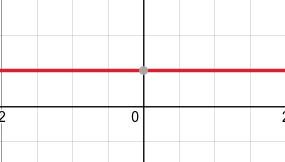
\includegraphics[width=\linewidth, height=2cm]{uniform.png} \caption{$f_{0}$} .
				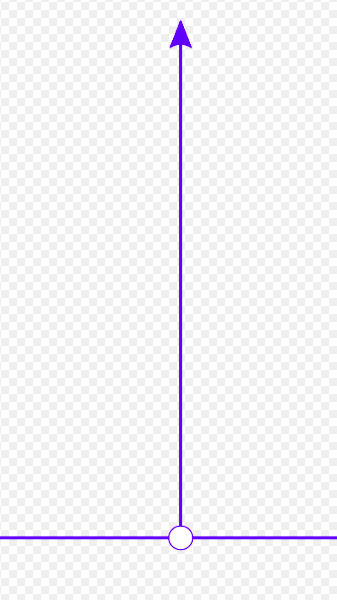
\includegraphics[width=\linewidth, height=2cm]{dirac.png} \caption{$f_{\delta}$}
			\end{multicols}
		\end{figure} 
	
		$f_{0}$ generated using desmos graphing calculator. $f_{\delta}$ snipped from the image in wikipedia for the Dirac delta function.
		
		\begin{itemize}
			\item Uniform and delta distributions are not very realistic in a system of large number of particles. 
			\item Parabolic functions in a given range are better and yet simple to work with.
		\end{itemize}
		
		
	\end{frame}

	\begin{frame}[t]{4.2 Parabolic density functions as approximation to Maxwellian}
	
	\[f_{1} =
	\begin{cases} 
		1- \frac{v^{2}}{2 v_{a}^2} & -v_{a}\leq v\leq v_{a} \\
		0 & else 
	\end{cases}
	\]
	\[ f_{2} = 
	\begin{cases}
		1 + \frac{v^{2}}{2 v_{a}^2} & -v_{a}\leq v\leq v_{a} \\
		0 & else
	\end{cases}\]

	These functions can be normalized as
	$$ \int_{v_{x} = -v_{a}}^{v_{x} = v_{a}} dv_{x} \int_{v_{y} = -v_{a}}^{v_{y} = v_{a}} dv_{y} \int_{v_{z} = -v_{a}}^{v_{z} = v_{a}} dv_{z} \hspace{0.2cm}c_{0}  \left(1 - \frac{v_{x}^{2}+v_{y}^{2}+v_{z}^{2}}{2 v_{a}^2}\right) = 1 \hspace{2cm} \mathrm{and}$$
	$$ \int_{v_{x} = -v_{a}}^{v_{x} = v_{a}} dv_{x} \int_{v_{y} = -v_{a}}^{v_{y} = v_{a}} dv_{y} \int_{v_{z} = -v_{a}}^{v_{z} = v_{a}} dv_{z} \hspace{0.2cm} c_{0}  \left(1 + \frac{v_{x}^{2}+v_{y}^{2}+v_{z}^{2}}{2 v_{a}^2}\right) = 1 \hspace{2cm} \mathrm{giving}$$

	\end{frame}

	\begin{frame}[t]{Parabolic density functions - Normalized}
		\[ \hat{f_{1}} = 
		\begin{cases} 
			\frac{1}{4 v_{a}^{3}} \left(1 - \frac{v^{2}}{2 v_{a}^2}\right) & -v_{a}\leq v\leq v_{a} \\
			0 & else 
		\end{cases}
		\]
		\[ \hat{f_{2}} = 
		\begin{cases}
			\frac{1}{12 v_{a}^{3}} \left(1 + \frac{v^{2}}{2 v_{a}^2}\right) & v_{a}\leq v\leq v_{a} \\
			0 & else
		\end{cases}\]
	
		\begin{multicols}{2}
			
			\begin{figure}[H]
			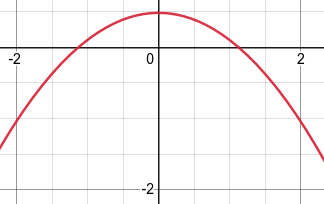
\includegraphics[width=\columnwidth, height=2cm]{first.png} \caption{$\hat{f_{1}}$} .
			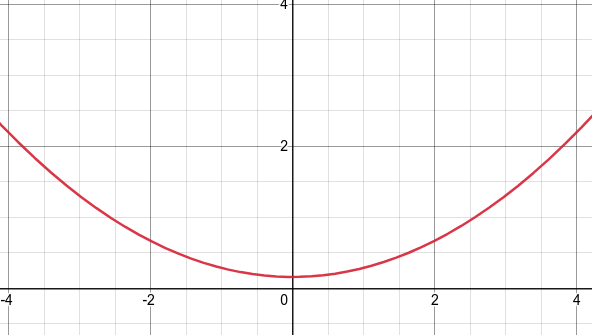
\includegraphics[width=\columnwidth, height=2cm]{second.png} \caption{$\hat{f_{2}}$}
			\end{figure}
		\end{multicols}
	

	\end{frame}
	
	\begin{frame}[t]{4.3 $\hat{f_{1}}$ , $\hat{f_{2}}$ and $\widehat{f_{M}}$ in  the collisionless Vlasov equation}
		Plugging in  $\hat{f_{1}}$ , $\hat{f_{2}}$ and $\widehat{f_{M}}$ in  the collisionless Vlasov equation
		$$ \frac{\partial f}{\partial t} + \textbf{v} \cdot \nabla f + \frac{q}{m} \left(\mathrm{\textbf{E}}+\textbf{v} \times \mathrm{\textbf{B}} \right) \cdot {\partial}_{\textbf{v}} f = 0 $$
		For all three of the density functions
		$$\frac{\displaystyle \partial f}{\displaystyle \partial t} = 0 \mathrm{,} \hspace{1cm} \frac{\displaystyle \partial f}{\displaystyle \partial x} = 0 \mathrm{,} \hspace{1cm} \frac{\displaystyle \partial f}{\displaystyle \partial y} = 0 \mathrm{,} \hspace{1cm} \frac{\displaystyle \partial f}{\displaystyle \partial z} = 0 $$ as all three have no explicit dependence on position or time. The Vlasov equation then becomes $$ \left(\mathrm{\textbf{E}}+\textbf{v} \times \mathrm{\textbf{B}} \right) \cdot {\partial}_{\textbf{v}} f = 0 $$ which is
		$$ \left(E_{x} + v_{y} B_{z} - v_{z} B_{y}\right) \frac{\displaystyle \partial f}{\displaystyle \partial v_{x}} + \left(E_{y} + v_{z} B_{x} - v_{x} B_{z}\right) \frac{\displaystyle \partial f}{\displaystyle \partial v_{y}} + $$ $$\left(E_{z} + v_{x} B_{y} - v_{y} B_{x}\right) \frac{\displaystyle \partial f}{\displaystyle \partial v_{z}} = 0$$
		
	\end{frame}
	
	\begin{frame}[t]{$\widehat{f_{M}}$ in  the collisionless Vlasov equation}
		For the Maxwellian, $$ 	\widehat{f_{M}} := \hat{f}(\textbf{r}, \textbf{v}, t) = \left(\frac{m}{2\pi KT}\right)^{\frac{3}{2}} exp \left(-\frac{v^{2}}{v_{th}^{2}}\right) $$
		$$\frac{\displaystyle \partial f_{M}}{\displaystyle \partial v_{x}} = \left(\frac{m}{2 \pi K T}\right)^{\frac{3}{2}}  exp \left(\frac{-v^{2}}{v_{th}^{2}}\right)\left(\frac{-2 v_{x}}{v_{th}^{2}}\right)$$ $$ \frac{\displaystyle \partial f_{M}}{\displaystyle \partial v_{y}} = \left(\frac{m}{2 \pi K T}\right)^{\frac{3}{2}}  exp  \left(\frac{-v^{2}}{v_{th}^{2}}\right)\left(\frac{-2 v_{y}}{v_{th}^{2}}\right)$$ $$\frac{\displaystyle \partial f_{M}}{\displaystyle \partial v_{z}} = \left(\frac{m}{2 \pi K T}\right)^{\frac{3}{2}}  exp  \left(\frac{-v^{2}}{v_{th}^{2}}\right)\left(\frac{-2 v_{z}}{v_{th}^{2}}\right)$$
		plugging in, the equation becomes
		$$\left(\frac{m}{2 \pi K T}\right)^{\frac{3}{2}}  exp  \left(\frac{-v^{2}}{v_{th}^{2}}\right)\left(\frac{-2}{v_{th}^{2}}\right) \left[v_{x}\left( E_{x} + v_{y} B_{z} - v_{z} B_{y} \right) + \right. $$ $$v_{y} \left( E_{y} + v_{z} B_{x} - v_{x} B_{z} \right) + \left. v_{z} \left(E_{z} + v_{x} B_{y} - v_{y} B_{x}\right) \right] = 0$$
		
	\end{frame}

	\begin{frame}[t]{$\widehat{f_{M}}$ in  the collisionless Vlasov equation}
		which gives
		$$v_{x} E_{x} + v_{y} E{y} + v_{z} E_{z} = 0$$
		which can also be written as 
		\begin{equation}
			\label{eqn:MaxwellInVlasov}
			\textbf{v} \cdot \mathrm{\textbf{E}} = 0
		\end{equation} 
		which says that the particles move perpendicular to the electric field which is characteristic of the Lorentz force.\\
	For the parabolic functions,
	\[ \hat{f_{1}} = 
	\begin{cases} 
		\frac{1}{4 v_{a}^{3}} \left(1 - \frac{v^{2}}{2 v_{a}^2}\right) & -v_{a}\leq v\leq v_{a} \\
		0 & else 
	\end{cases}
	\]
	\[ \hat{f_{2}} = 
	\begin{cases}
		\frac{1}{12 v_{a}^{3}} \left(1 + \frac{v^{2}}{2 v_{a}^2}\right) & v_{a}\leq v\leq v_{a} \\
		0 & else
	\end{cases}\]
	\end{frame}

	\begin{frame}[t]{$\hat{f_{1}}$ and $\hat{f_{2}}$ in  the collisionless Vlasov equation}
	\[ \frac{\displaystyle \partial \hat{f_{1}}}{\displaystyle \partial v_{x}} = 
	\begin{cases} 
		\frac{1}{4 v_{a}^{3}} \left(\frac{- 2 v_{x}}{2 v_{a}^2}\right) & -v_{a} < v < v_{a} \\
		undefined & v = - v_{a}, v = v_{a} \\
		0 & else 
	\end{cases}
	\]
	\[ \frac{\displaystyle \partial \hat{f_{1}}}{\displaystyle \partial v_{y}} = 
	\begin{cases} 
		\frac{1}{4 v_{a}^{3}} \left(\frac{- 2 v_{y}}{2 v_{a}^2}\right) & -v_{a} < v < v_{a} \\
		undefined & v = - v_{a}, v = v_{a} \\
		0 & else 
	\end{cases}
	\]
	\[ \frac{\displaystyle \partial \hat{f_{1}}}{\displaystyle \partial v_{z}} = 
	\begin{cases} 
		\frac{1}{4 v_{a}^{3}} \left(\frac{- 2 v_{z}}{2 v_{a}^2}\right) & -v_{a} < v < v_{a} \\
		undefined & v = - v_{a}, v = v_{a} \\
		0 & else 
	\end{cases}
	\]
	
	
	\end{frame}

	\begin{frame}
		\[ \frac{\displaystyle \partial \hat{f_{2}}}{\displaystyle \partial v_{x}} = 
		\begin{cases} 
			\frac{1}{12 v_{a}^{3}} \left(\frac{2 v_{x}}{2 v_{a}^2}\right) & -v_{a} < v < v_{a} \\
			undefined & v = - v_{a}, v = v_{a} \\
			0 & else 
		\end{cases}
		\]
		\[ \frac{\displaystyle \partial \hat{f_{2}}}{\displaystyle \partial v_{y}} = 
		\begin{cases} 
			\frac{1}{12 v_{a}^{3}} \left(\frac{2 v_{y}}{2 v_{a}^2}\right) & -v_{a} < v < v_{a} \\
			undefined & v = - v_{a}, v = v_{a} \\
			0 & else 
		\end{cases}
		\]
		\[ \frac{\displaystyle \partial \hat{f_{2}}}{\displaystyle \partial v_{z}} = 
		\begin{cases} 
			\frac{1}{12 v_{a}^{3}} \left(\frac{2 v_{z}}{2 v_{a}^2}\right) & -v_{a} < v < v_{a} \\
			undefined & v = - v_{a}, v = v_{a} \\
			0 & else 
		\end{cases}
		\]
	\end{frame}
	
	\begin{frame}
		In the range $v \in \mathbb{R} \textbackslash \left[-v_{a}, v_{a}\right] $ the equation becomes $0 = 0$ which is trivial. The equation becomes undefined for $v = v_{a}$ and 
		$v = - v_{a}$ but we can ignore that for now. In the interesting range of $v \in \left(-v_{a}, v_{a}\right) $, the equation becomes 
		$$ \frac{1}{4 v_{a}^{3}} \left(\frac{- 2}{2 v_{a}^2}\right) \left[v_{x}\left( E_{x} + v_{y} B_{z} - v_{z} B_{y} \right) + v_{y} \left(E_{y} + v_{z} B_{x} - v_{x} B_{z} \right) + \right. $$ $$\left. v_{z} \left(E_{z} + v_{x} B_{y} - v_{y} B_{x}\right) \right] = 0 $$
		for $\hat{f_{1}}$ and
		$$ \frac{1}{12 v_{a}^{3}} \left(\frac{2}{2 v_{a}^2}\right) \left[v_{x}\left( E_{x} + v_{y} B_{z} - v_{z} B_{y} \right) + v_{y} \left( E_{y} + v_{z} B_{x} - v_{x} B_{z} \right) + \right. $$ $$\left. v_{z} \left(E_{z} + v_{x} B_{y} - v_{y} B_{x}\right) \right] = 0 $$
		for $\hat{f_{2}}$ which both give
		$$v_{x} E_{x} + v_{y} E{y} + v_{z} E_{z} = 0 \hspace{1cm}\mathrm{or}\hspace{1cm}\textbf{v} \cdot \mathrm{\textbf{E}} = 0$$
		\noindent $\hat{f_{1}}$ and $\hat{f_{2}}$ behave similar to $\hat{f_{M}}$ when plugged into the Vlasov equation.
		
	\end{frame}

	\begin{frame}[t]{4.4 Plugging into the expression for Magnetic Mirror}
			\noindent Since the quantity $\frac{\displaystyle sin^{2}\theta}{\displaystyle B_{z}}$ is conserved in a magnetic mirror, it is a good exercise to calculate the average value or expectation of $sin^{2}\theta$, $\left\langle sin^{2}\theta\right\rangle = \left\langle \frac{\displaystyle v_{\perp}^{2}}{\displaystyle v^{2}}\right\rangle = \left\langle \frac{\displaystyle v_{x}^{2} + v_{y}^{2}}{\displaystyle v_{x}^{2} + v_{y}^{2} +  v_{z}^{2}}\right\rangle $ 
			
			For the Maxwellian $\widehat{f_{M}}$,
			$$\left\langle \frac{\displaystyle v_{x}^{2} + v_{y}^{2}}{\displaystyle v_{x}^{2} + v_{y}^{2} +  v_{z}^{2}}\right\rangle = \left(\frac{m}{2\pi KT}\right)^{\frac{3}{2}} $$ 
			$$ \int_{v_{x} = - \infty}^{v_{x} = \infty} d v_{x} \int_{v_{y} = - \infty}^{v_{y} = \infty} d v_{y} \int_{v_{z} = - \infty}^{v_{z} = \infty} d v_{z} \left( \frac{\displaystyle v_{x}^{2} + v_{y}^{2}}{\displaystyle v_{x}^{2} + v_{y}^{2} + v_{z}^{2}} \right)  exp \left(-\frac{v_{x}^{2}}{v_{th}^{2}}\right) $$ $$ exp \left(-\frac{v_{y}^{2}}{v_{th}^{2}}\right) exp\left(-\frac{v_{z}^{2}}{v_{th}^{2}}\right)$$
		
	\end{frame}

	\begin{frame}
		for $\hat{f_{1}}$
		$$\left\langle \frac{\displaystyle v_{x}^{2} + v_{y}^{2}}{\displaystyle v_{x}^{2} + v_{y}^{2} +  v_{z}^{2}}\right\rangle = \frac{1}{4 v_{a}^{3}} $$ $$\int_{v_{x} = - v_{a}}^{v_{x} = v_{a}} d v_{x} \int_{v_{y} = - v_{a}}^{v_{y} = v_{a}} d v_{y} \int_{v_{z} = - v_{a}}^{v_{z} = v_{a}} d v_{z} \left( \frac{\displaystyle v_{x}^{2} + v_{y}^{2}}{\displaystyle v_{x}^{2} + v_{y}^{2} + v_{z}^{2}} \right)$$ $$  \left(1 - \frac{v_{x}^{2}}{2 v_{a}^2} - \frac{v_{y}^{2}}{2 v_{a}^2} - \frac{v_{z}^{2}}{2 v_{a}^2} \right) $$
		for $\hat{f_{2}}$
		$$\left\langle \frac{\displaystyle v_{x}^{2} + v_{y}^{2}}{\displaystyle v_{x}^{2} + v_{y}^{2} +  v_{z}^{2}}\right\rangle = \frac{1}{12 v_{a}^{3}} $$ $$\int_{v_{x} = - v_{a}}^{v_{x} = v_{a}} d v_{x} \int_{v_{y} = - v_{a}}^{v_{y} = v_{a}} d v_{y} \int_{v_{z} = - v_{a}}^{v_{z} = v_{a}} d v_{z} \left( \frac{\displaystyle v_{x}^{2} + v_{y}^{2}}{\displaystyle v_{x}^{2} + v_{y}^{2} + v_{z}^{2}} \right) $$ $$ \left(1 + \frac{v_{x}^{2}}{2 v_{a}^2} + \frac{v_{y}^{2}}{2 v_{a}^2} + \frac{v_{z}^{2}}{2 v_{a}^2} \right) $$
		
	\end{frame}

	\begin{frame}
		Integrals are \textbf{Very Difficult!} to evaluate because of the denominators. \\
		\noindent So an approximation $\left\langle \frac{\displaystyle v_{x}^{2} + v_{y}^{2}}{\displaystyle v_{x}^{2} + v_{y}^{2} +  v_{z}^{2}}\right\rangle =  \frac{\displaystyle \left\langle v_{x}^{2} + v_{y}^{2}\right\rangle}  {\displaystyle \left\langle v_{x}^{2} + v_{y}^{2} +  v_{z}^{2}\right\rangle} + c_{0}$ can be done where $c_{0}$ is an error term.\\
		
		\noindent For $\widehat{f_{M}}$, $\displaystyle \left\langle v_{x}^{2} + v_{y}^{2}\right\rangle = \frac{\displaystyle 2 K T}{\displaystyle m}$ and $\left\langle v_{x}^{2} + v_{y}^{2} +  v_{z}^{2}\right\rangle = \frac{\displaystyle 3 K T}{\displaystyle m}$ so $$\left\langle sin^{2}\theta\right\rangle = \left\langle \frac{\displaystyle v_{\perp}^{2}}{\displaystyle v^{2}}\right\rangle = \left\langle \frac{\displaystyle v_{x}^{2} + v_{y}^{2}}{\displaystyle v_{x}^{2} + v_{y}^{2} +  v_{z}^{2}}\right\rangle = \frac{\displaystyle \left\langle v_{x}^{2} + v_{y}^{2}\right\rangle}  {\displaystyle \left\langle v_{x}^{2} + v_{y}^{2} +  v_{z}^{2}\right\rangle} + c_{0} = \frac{2}{3} + c_{0}$$
		For $\hat{f_{1}}$, $\displaystyle \left\langle v_{x}^{2} + v_{y}^{2}\right\rangle = \frac{22}{45} v_{a}^2$ and $\displaystyle \left\langle v_{x}^{2} + v_{y}^{2} +  v_{z}^{2}\right\rangle = \frac{11}{15} v_{a}^2$ so $\displaystyle \left\langle sin^{2}\theta\right\rangle = \frac{2}{3} + c_{0}$ and \vspace{0.2cm} \\
		\noindent For $\hat{f_{2}}$, $\displaystyle \left\langle v_{x}^{2} + v_{y}^{2}\right\rangle = \frac{98}{135} v_{a}^2$ and $\displaystyle \left\langle v_{x}^{2} + v_{y}^{2} +  v_{z}^{2}\right\rangle = \frac{49}{45} v_{a}^2$ so $\displaystyle \left\langle sin^{2}\theta\right\rangle = \frac{2}{3} + c_{0}$ \\
		
	\end{frame}

	\begin{frame}
		\noindent 
		\begin{itemize}
			\item $\hat{f_{1}}$ and $\hat{f_{2}}$ behave similar to $\widehat{f_{M}}$ when plugged into the Vlasov equation
			\item $\hat{f_{1}}$ and $\hat{f_{2}}$ behave similar to $\widehat{f_{M}}$ when plugged into the expression for $\left\langle sin^{2}\theta\right\rangle$
			\item \textbf{Hence!} $\hat{f_{1}}$ and $\hat{f_{2}}$ are nice distribution functions to work with as an approximation to $\widehat{f_{M}}$.
	\end{itemize}
	\end{frame}

	\begin{frame}[t]{5. Vlasov - Poisson}
		
	\end{frame}

	\begin{frame}[t]{6. Particle in a cell}
		
	\end{frame}

	\begin{frame}[t]{References}
		\begin{thebibliography}{}
			\bibitem{chenbook}
			Chen, F. F. (1984). \textit{Introduction to plasma physics and controlled fusion} (Vol. 1, pp. 8-11). New York: Plenum press.
			\bibitem{mirror1}
			Na, Yong-Su (2017). \textit{Introduction to nuclear fusion} (Lecture 9 Mirror, lecture slide). Seoul National University Open Courseware.
			\bibitem{mirror2}
			F\"{o}rel\"{a}sning (2009). \textit{Charged particle motion in magnetic field} (lecture slide). Lule\"{a} University of Technology.
			
		\end{thebibliography}
	\end{frame}

\end{document}